\documentclass{article}

% NeurIPS 2026 preprint template.
\PassOptionsToPackage{numbers,compress}{natbib}
\PassOptionsToPackage{hidelinks}{hyperref}
\usepackage[preprint]{neurips_2026}

\usepackage[utf8]{inputenc}
\usepackage[T1]{fontenc}
\usepackage{microtype}
\usepackage{amsmath,amssymb}
\usepackage{booktabs}
\usepackage{enumitem}
\usepackage{graphicx}
\usepackage{tabularx}
\usepackage{multirow}
\usepackage{xcolor}
\usepackage{hyperref}

\title{Compression Safety in Biomedical Vision Models\\
Clinical Evaluation of Pruning, Quantization, and Distillation on HAM10000}

\author{%
  Abdulla Alfalasi \\
  ML8505 --- Tiny Machine Learning \\
  Mohamed Bin Zayed University of AI \\
  \And
  Mohammed Ibrahim \\
  ML8505 --- Tiny Machine Learning \\
  Mohamed Bin Zayed University of AI \\
}
\date{}

\newcommand{\mel}{\ensuremath{\textit{mel}}}
\newcommand{\bcc}{\ensuremath{\textit{bcc}}}
\newcommand{\akiec}{\ensuremath{\textit{akiec}}}
\newcommand{\nv}{\ensuremath{\textit{nv}}}
\newcommand{\DCR}{\ensuremath{\mathrm{DCR}}}

\begin{document}
\maketitle

\begin{abstract}
Compression studies for medical imaging usually report a single accuracy number. That hides the question clinicians actually care about: are the rare dangerous classes still detected, and is the model's confidence still trustworthy? We answer this for skin lesion classification on HAM10000 with DeiT-Tiny and DeiT-Small.

We compare four pruning rules (magnitude, Wanda, Taylor, random), sensitivity-guided non-uniform sparsity, INT8 post-training quantization, and knowledge distillation. Alongside balanced accuracy, melanoma AUROC, ECE, and model size, we report a Dangerous-Class Degradation Ratio (\DCR{}) that measures how much performance drops on the three dangerous lesion classes (melanoma, basal cell carcinoma, and actinic keratosis) relative to the safer classes.

Four findings stand out. (i) Magnitude pruning is the least safe baseline: it has the highest \DCR{} and loses dangerous-class recall first. (ii) Taylor pruning at 50\% sparsity gives the best clinical tradeoff, with strong melanoma discrimination and low calibration error; this ordering holds across the 20--70\% sweep, and a per-layer gradient-flow analysis explains why. (iii) INT8 quantization preserves dense-model behavior and cuts size by 3.8$\times$. (iv) Non-uniform sparsity can rescue Wanda when recall matters, but it shifts the error profile and needs calibration-aware validation; distillation helps the dense student but does not make it more robust to pruning.

The contribution is a deployment-oriented evaluation protocol and recommendation set for biomedical vision models, not a new compression technique.
\end{abstract}

\section{Introduction}
Biomedical vision models are attractive precisely where deployment is most constrained: dermatology screening in low-connectivity clinics, point-of-care triage, and mobile or edge-assisted second reads. In these settings, memory footprint, latency, and privacy all matter. Compression is therefore not a cosmetic optimization. It is the mechanism that makes the model deployable.

The problem is that conventional evaluation hides the failure mode that matters most clinically. HAM10000 is strongly imbalanced, with \nv{} dominating the dataset and melanoma, basal cell carcinoma, and actinic keratosis appearing much less often. A compressed model can preserve balanced accuracy while silently degrading the classes a clinician cares about most. That failure is especially dangerous because it can look like progress if one only reports a single aggregate number.

This paper asks a practical question: when a medical Vision Transformer is compressed, which choices preserve diagnostic safety, and which merely preserve headline metrics? We treat this as a deployment problem rather than a novelty problem. The contribution is an evaluation protocol that exposes class-asymmetric failure, plus a set of recommendations for biomedical teams that want to compress models without introducing avoidable risk.

Our main contributions are:
\begin{itemize}[leftmargin=*,itemsep=2pt,topsep=2pt]
\item We introduce \DCR{}, a compact safety metric that measures whether compression harms dangerous lesions more than safer ones.
\item We run lesion-grouped, multi-seed pruning comparisons on DeiT-Tiny and DeiT-Small across the full 20--70\% sparsity sweep, and show that magnitude is the least safe baseline while Taylor is the strongest sparse default.
\item We quantify attention overlap against lesion masks and show that Wanda's failure is downstream of attention, not a failure to localize lesions.
\item We add a gradient-flow mechanism probe that explains magnitude's class-asymmetric damage and explicitly reject the simpler activation-concentration hypothesis.
\item We restore the deployment-oriented experiments that matter to biomedical integrators: non-uniform sparsity, INT8 stacking, knowledge distillation, recovery fine-tuning, calibration-size ablation, and a MobileNetV2 baseline.
\item We turn those results into a practical recommendation set: use lesion-grouped splits, report AUROC and calibration alongside sensitivity, start with INT8, use Taylor rather than magnitude when sparsity is required, and treat every evaluated pipeline as academic-only unless it clears the conservative clinical thresholds.
\end{itemize}

\section{Related Work}
\paragraph{Pruning and sparsity.}
Magnitude pruning \cite{han2015deep} remains the standard baseline because it is simple and cheap to compute. Taylor scoring \cite{molchanov2017taylor} adds task sensitivity by accounting for the loss gradient. Wanda \cite{sun2023wanda} extends activation-aware pruning ideas from language models to vision by combining weight magnitude and activation norm. In biomedical settings, pruning is often evaluated primarily on aggregate accuracy, which is not enough to characterize class-specific safety.

\paragraph{Quantization and distillation.}
INT8 post-training quantization is a mature deployment technique with a well-understood efficiency tradeoff \cite{jacob2018quantization,gholami2021survey}. Knowledge distillation \cite{hinton2015distillation} and DeiT-style training \cite{touvron2021deit} can improve dense model quality, but it is not obvious that a better dense student is also a more pruning-robust student.

\paragraph{Medical evaluation.}
Recent work on medical pruning and explainability emphasizes fairness, interpretability, or sparsity quality \cite{paxton2025,yu2023xpruner}. Our focus is narrower and more deployment-oriented: we ask whether compression changes the diagnostic operating point in ways that matter for lesion triage, referral, and screening.

\paragraph{Attention analysis.}
Attention rollout and attention-flow metrics \cite{abnar2020attention} are often used qualitatively. We use them here in a more conservative way: as a check on whether pruning destroys lesion localization or whether the observed failure happens later in the pipeline.

\section{Method}
\paragraph{Dataset and splits.}
We use HAM10000 \cite{tschandl2018ham10000}, which contains 10{,}015 dermoscopic images across seven classes: \akiec{}, \bcc{}, \textit{bkl}, \textit{df}, \mel{}, \nv{}, and \textit{vasc}. Splits are constructed with lesion-grouped \texttt{GroupShuffleSplit} on \texttt{lesion\_id}, so every lesion is assigned entirely to train or validation. This matters: image-level splitting would leak lesion-specific cues and inflate the reported metrics.

\paragraph{Models and compression.}
We fine-tune DeiT-Tiny and DeiT-Small from \texttt{timm}. DeiT-Small also serves as the teacher in the distillation follow-up. We compare four one-shot pruning criteria at multiple sparsities: magnitude, Wanda, Taylor, and random. We additionally evaluate sensitivity-guided non-uniform sparsity, INT8 post-training quantization, knowledge distillation as a pre-treatment, post-pruning recovery fine-tuning, calibration-size ablation, and a MobileNetV2 baseline.

\paragraph{Clinical metrics.}
We report balanced accuracy, per-class sensitivity, melanoma AUROC, macro AUROC, ECE, model size, and latency. The additional safety metric is the dangerous-class degradation ratio:
\begin{equation}
\DCR = \frac{\frac{1}{|\mathcal{D}|}\sum_{c \in \mathcal{D}}\left[\mathrm{Sens}^{\text{dense}}_c - \mathrm{Sens}^{\text{comp}}_c\right]}{\frac{1}{|\mathcal{S}|}\sum_{c \in \mathcal{S}}\left[\mathrm{Sens}^{\text{dense}}_c - \mathrm{Sens}^{\text{comp}}_c\right]},
\end{equation}
where $\mathcal{D}=\{\mel,\bcc,\akiec\}$ and $\mathcal{S}=\{\nv,\textit{bkl},\textit{df},\textit{vasc}\}$. Values above 1 mean compression hurts dangerous classes more than safer ones.

\paragraph{Protocol.}
Headline pruning results are reported as mean $\pm$ standard deviation across the available seeds. Where we compare methods directly, we use paired tests on matched seeds. The main pruning comparison centers on 50\% sparsity because that is the most informative tradeoff point for biomedical deployment.

\paragraph{Clinical regime tagging.}
Each aggregated run is also mapped to one of four conservative clinical regimes: \texttt{triage\_screen}, \texttt{specialist\_referral}, \texttt{primary\_diagnosis}, or \texttt{academic\_only}. These tags are derived from the log companion files and are intentionally strict. In the present study, every evaluated pipeline remains \texttt{academic\_only}, which is the right reading for a research paper: the goal is to quantify compression safety, not to overclaim clinical readiness.

\section{Results}

\subsection{Pruning criteria at 50\% sparsity}
Table~\ref{tab:headline} summarizes the main pruning comparison. The ranking that matters for biomedical deployment is clear: magnitude is the least safe baseline, Taylor gives the strongest sparse tradeoff, and Wanda has the worst calibration even when it preserves some recall.

\begin{table*}[t]
\centering
\small
\caption{Headline pruning results at 50\% sparsity. The key biomedical question is not only which method keeps average performance high, but which one avoids preferentially forgetting dangerous classes. Dense baselines are shown for reference.}
\label{tab:headline}
\resizebox{\textwidth}{!}{%
\begin{tabular}{llccccccc}
\toprule
Model & Criterion & Bal.\ Acc. & Mel.\ Sens. & Mel.\ AUROC & Macro AUROC & ECE & \DCR & Spec@90Sens \\
\midrule
\multirow{5}{*}{DeiT-Small}
 & Dense       & $0.914 \pm 0.032$ & $0.896 \pm 0.030$ & $0.964 \pm 0.010$ & $0.986 \pm 0.008$ & $0.017 \pm 0.009$ & --- & $0.905 \pm 0.031$ \\
 & Magnitude   & $0.789 \pm 0.026$ & $0.571 \pm 0.052$ & $0.881 \pm 0.018$ & $0.959 \pm 0.007$ & $0.035 \pm 0.008$ & $1.89 \pm 0.42$ & $0.663 \pm 0.029$ \\
 & Wanda       & $0.612 \pm 0.018$ & $0.541 \pm 0.042$ & $0.837 \pm 0.018$ & $0.923 \pm 0.006$ & $0.099 \pm 0.005$ & $0.77 \pm 0.09$ & $0.568 \pm 0.044$ \\
 & Taylor      & $0.770 \pm 0.032$ & $0.843 \pm 0.031$ & $0.931 \pm 0.012$ & $0.973 \pm 0.006$ & $0.031 \pm 0.007$ & $0.95 \pm 0.26$ & $0.795 \pm 0.042$ \\
 & Random      & $0.133 \pm 0.011$ & $0.000 \pm 0.000$ & $0.523 \pm 0.049$ & $0.537 \pm 0.032$ & $0.249 \pm 0.125$ & $0.99 \pm 0.36$ & $0.170 \pm 0.028$ \\
\midrule
\multirow{5}{*}{DeiT-Tiny}
 & Dense       & $0.906 \pm 0.035$ & $0.845 \pm 0.038$ & $0.951 \pm 0.011$ & $0.984 \pm 0.005$ & $0.025 \pm 0.009$ & --- & $0.869 \pm 0.035$ \\
 & Magnitude   & $0.758 \pm 0.038$ & $0.518 \pm 0.048$ & $0.895 \pm 0.014$ & $0.960 \pm 0.006$ & $0.049 \pm 0.005$ & $3.83 \pm 1.66$ & $0.695 \pm 0.044$ \\
 & Wanda       & $0.338 \pm 0.010$ & $0.934 \pm 0.019$ & $0.799 \pm 0.024$ & $0.823 \pm 0.010$ & $0.118 \pm 0.006$ & $0.63 \pm 0.06$ & $0.558 \pm 0.045$ \\
 & Taylor      & $0.585 \pm 0.016$ & $0.814 \pm 0.121$ & $0.868 \pm 0.027$ & $0.942 \pm 0.007$ & $0.039 \pm 0.010$ & $0.99 \pm 0.18$ & $0.630 \pm 0.053$ \\
 & Random      & $0.140 \pm 0.006$ & $0.964 \pm 0.089$ & $0.482 \pm 0.080$ & $0.540 \pm 0.025$ & $0.148 \pm 0.038$ & $0.67 \pm 0.05$ & $0.168 \pm 0.077$ \\
\bottomrule
\end{tabular}}
\end{table*}

The key point is not that magnitude is always bad or that Wanda is always worse in the same way. The key point is that the failure mode changes with the scoring rule. Magnitude loses dangerous-class recall first on the larger backbone and has the highest \DCR{}. Wanda preserves some dangerous-class recall on DeiT-Small, but at the cost of much worse calibration and a markedly worse discrimination profile. Taylor is the only criterion that stays in the clinically useful part of the tradeoff curve on both backbones.

\subsection{Full sparsity sweep and significance}
Table~\ref{tab:headline} is the center point, not the whole story. The full 20--70\% sparsity sweep preserves the same ordering, but the shape of the failure changes with both backbone and criterion. At 20\% sparsity, all three criteria remain close to dense on DeiT-Small: magnitude reaches $0.920$ balanced accuracy with $0.908$ melanoma sensitivity, Wanda reaches $0.915$ / $0.870$, and Taylor reaches $0.915$ / $0.885$. By 40\%, the backbone split starts to matter. By 60--70\%, magnitude and Wanda leave the clinically useful frontier for different reasons, while Taylor is the only criterion that still preserves nontrivial discrimination on both backbones.

The paired tests confirm that the 50\% headline comparison is not a seed artifact. Wanda vs.\ magnitude balanced accuracy is highly significant on both backbones ($p < 10^{-15}$), but melanoma sensitivity does not move in the same direction across backbones: on DeiT-Small, magnitude slightly exceeds Wanda on melanoma sensitivity, while on DeiT-Tiny Wanda overshoots melanoma sensitivity by nearly $0.42$ and simultaneously collapses balanced accuracy. That is exactly why AUROC and ECE must remain in the table; sensitivity alone would make the smaller backbone look safer than it is.

At the edge of the sweep, the picture is even clearer. At 70\% sparsity, DeiT-Small magnitude and Wanda both lose melanoma sensitivity entirely, while Taylor still reports balanced accuracy above $0.42$ and melanoma sensitivity above $0.36$. On DeiT-Tiny, Wanda reaches melanoma sensitivity of $1.000$ at 70\%, but that number is a threshold artifact, not a clinical success: balanced accuracy is $0.143$ and ECE remains high. In other words, the full sweep does not change the ranking; it only shows how each criterion fails.

\begin{figure*}[t]
\centering
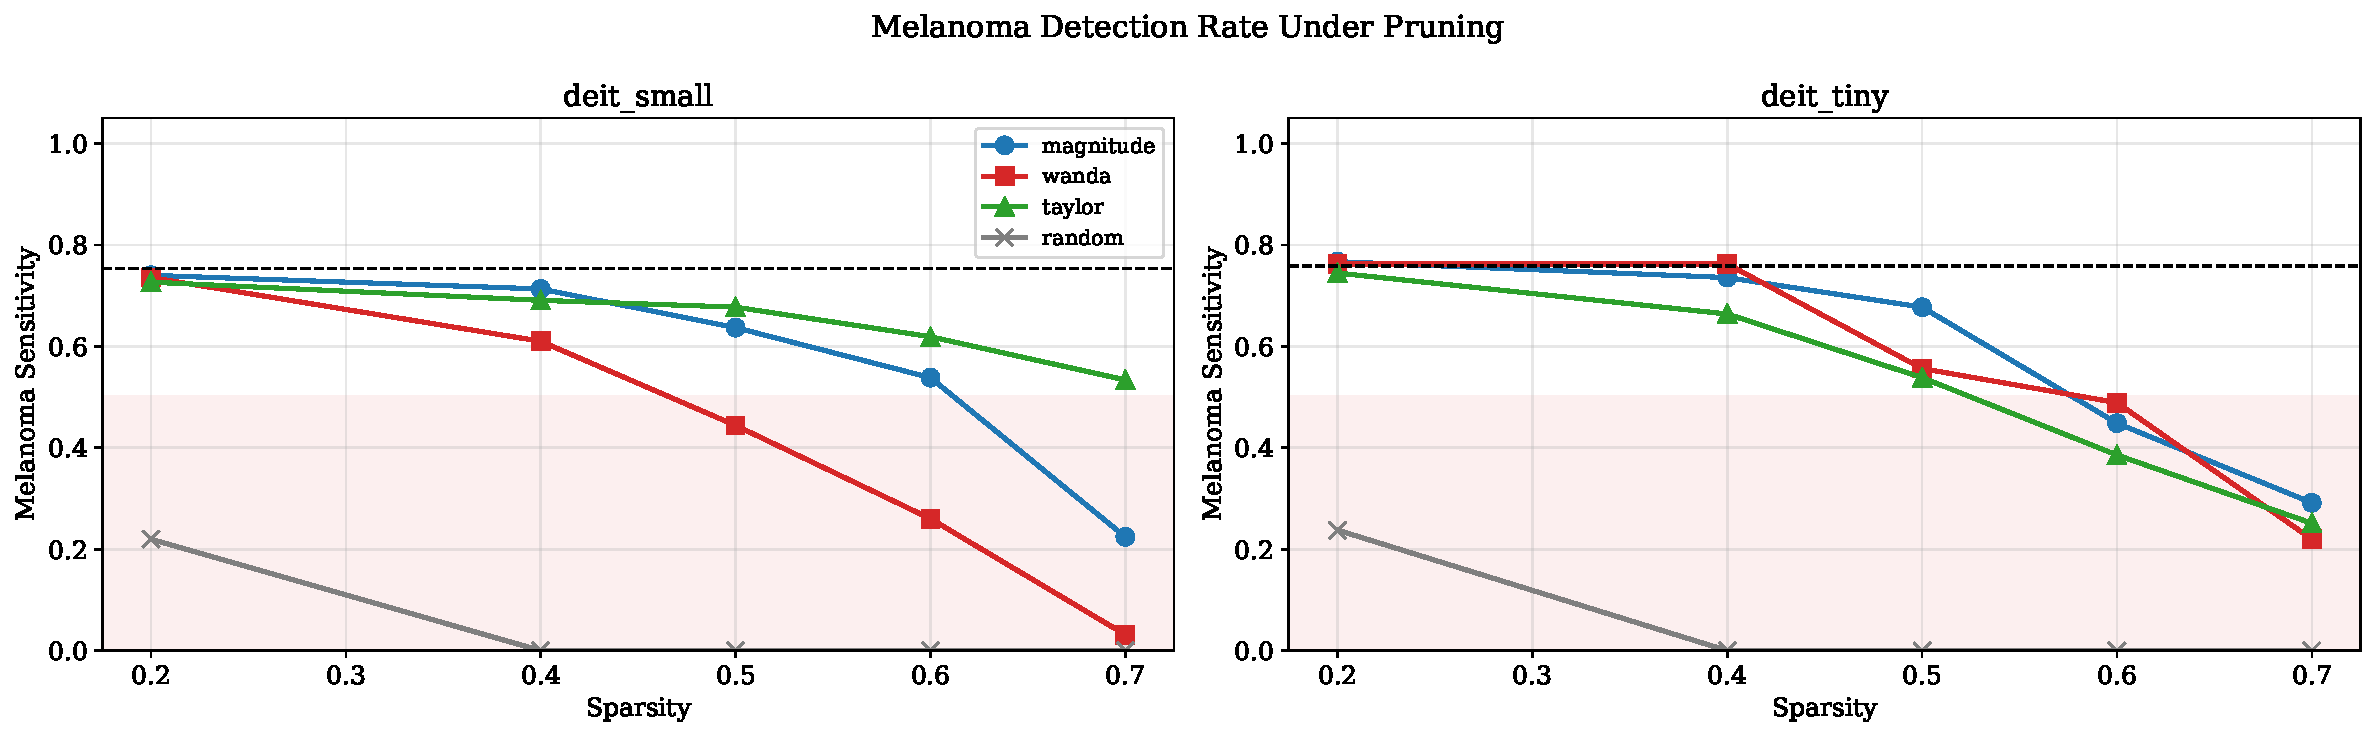
\includegraphics[width=0.49\textwidth]{../results/figures_local/fig1_melanoma_sensitivity.pdf}
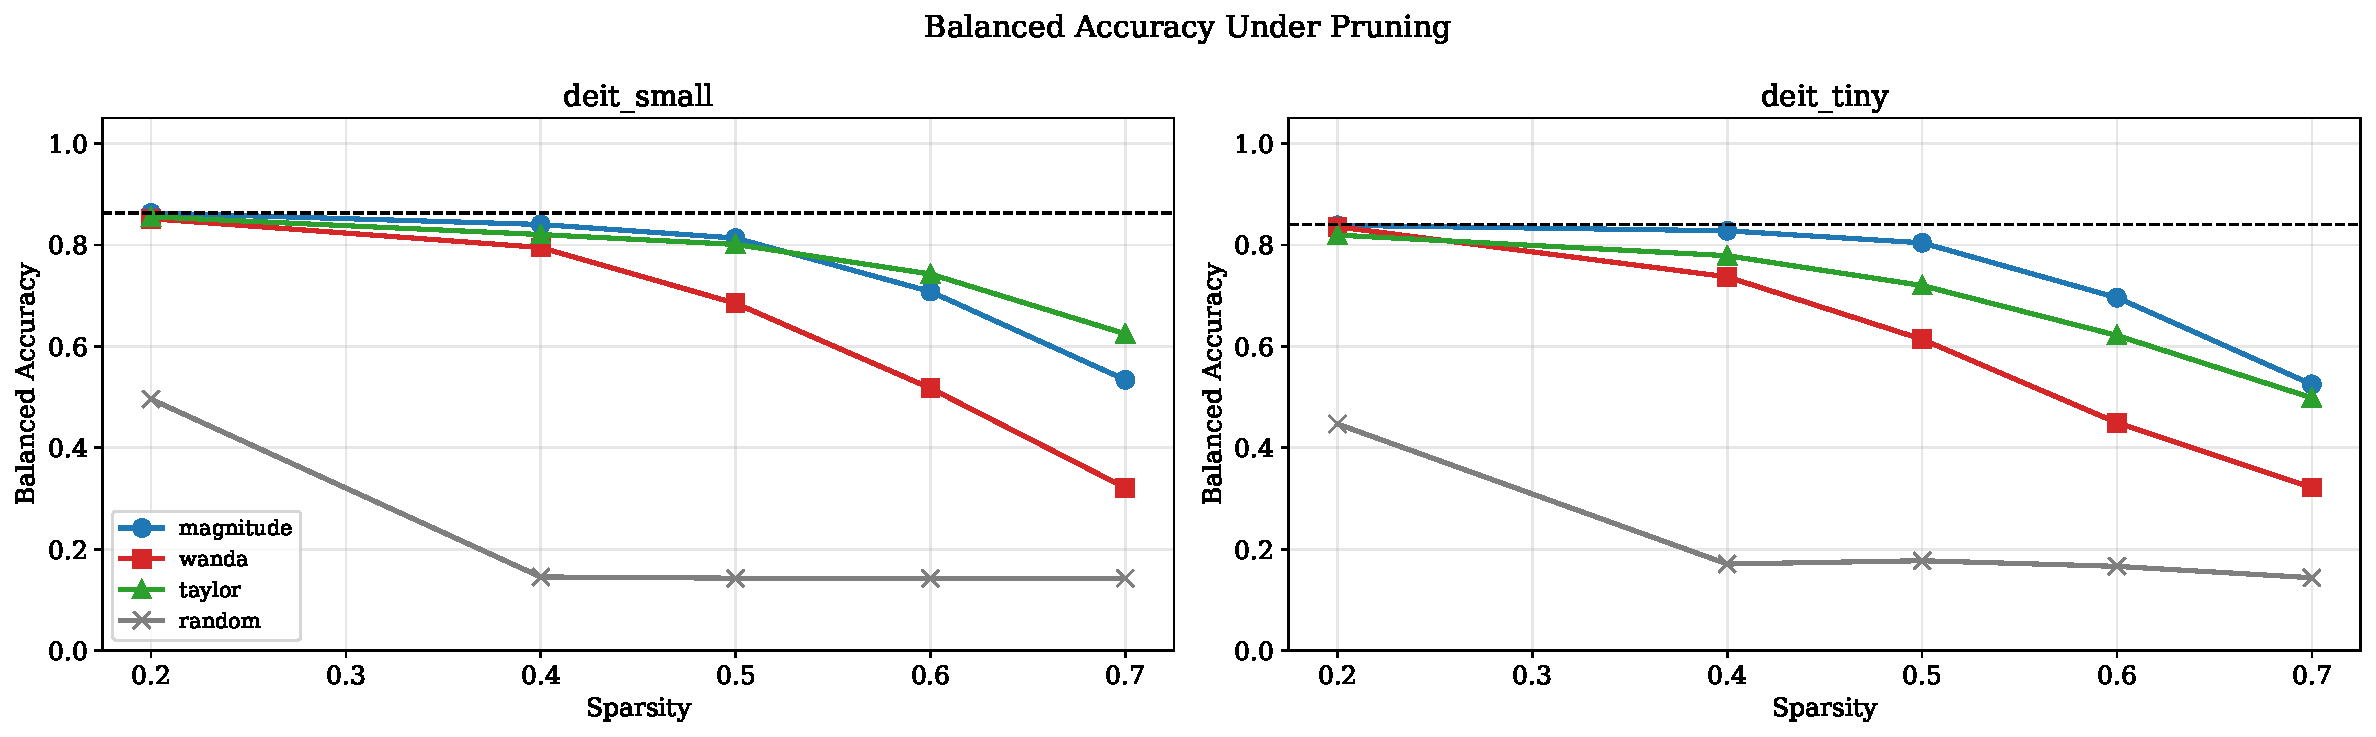
\includegraphics[width=0.49\textwidth]{../results/figures_local/fig2_balanced_accuracy.pdf}
\caption{Across-sparsity behavior from the project's exploratory run. The two views are complementary: melanoma sensitivity can rise even while balanced accuracy collapses, so sensitivity alone is not a sufficient safety signal. The sparse frontier remains most stable for Taylor, while Wanda's behavior is highly scale-dependent.}
\label{fig:sparsity_curves}
\end{figure*}

\subsection{Safety is not captured by sensitivity alone}
Figure~\ref{fig:sparsity_curves} is the main reason we report multiple metrics. On DeiT-Tiny, Wanda can inflate melanoma sensitivity even while collapsing balanced accuracy and AUROC. That is not a clinical improvement. It is a threshold shift. If we were to report only sensitivity, we would confuse over-prediction with discrimination.

That distinction matters for biomedical deployment. A screening model that over-calls melanoma may look safer in a sensitivity-only table, but it can become useless in practice because the false-positive burden becomes too high. AUROC and calibration are needed to separate genuine improvement from prediction collapse. Figure~\ref{fig:sens_vs_auroc} makes this concrete: every (backbone, criterion) point at 50\% sparsity is placed in the sensitivity-AUROC plane, and Wanda on DeiT-Tiny lands inside the shaded ``classifier collapse'' region (high sensitivity, low AUROC) while Taylor and the dense baselines stay in the upper-right, clinically useful corner.

\begin{figure}[t]
\centering
\includegraphics[width=\linewidth]{../results/figures_personal/fig_mel_sens_vs_auroc.pdf}
\caption{Melanoma sensitivity versus melanoma AUROC at 50\% sparsity. The shaded region marks classifier collapse, where high sensitivity coexists with low discrimination. Wanda on DeiT-Tiny falls inside this region, which is why a sensitivity-only report would misread it as the safest configuration.}
\label{fig:sens_vs_auroc}
\end{figure}

\begin{figure}[t]
\centering
\includegraphics[width=\linewidth]{../results/figures_personal/fig_dcr_bars.pdf}
\caption{Dangerous-Class Degradation Ratio on the available multi-seed personal aggregate. Magnitude prunes dangerous classes more aggressively than safer ones, while Wanda flips the direction of the imbalance. Taylor stays closest to a balanced tradeoff.}
\label{fig:dcrbars}
\end{figure}

\subsection{Why the criteria behave differently}
Figure~\ref{fig:dcrbars} makes the safety asymmetry explicit. Magnitude pruning is the clinically dangerous default because it preferentially removes weights that support the classes that were already underrepresented during fine-tuning. Wanda is different: it preserves a subset of high-activation features, but that does not guarantee better discrimination. In our results, Wanda's dangerous-class recall can look acceptable while the model's calibration degrades sharply.

Taylor behaves differently because it is sensitive to the loss gradient. In an imbalanced biomedical problem, the loss gradient already carries class information. That is why Taylor tends to keep the decision-critical layers intact. In other words, Taylor is not magically more sophisticated than magnitude; it is simply more aligned with the task.

\begin{figure}[t]
\centering
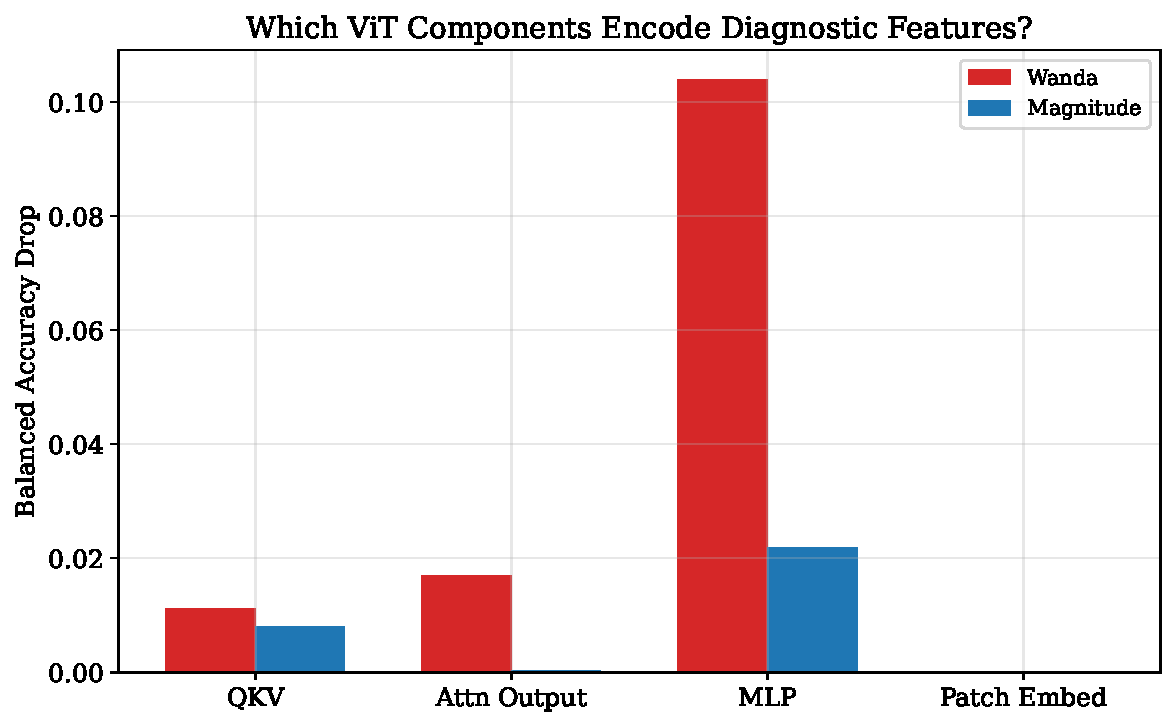
\includegraphics[width=\linewidth]{../results/figures_local/fig3_perlayer_bars.pdf}
\caption{Exploratory per-layer analysis from the local run. The bars show which ViT components lose the most balanced accuracy when individually pruned. The MLP blocks are the main sensitivity hotspot, while patch embedding is comparatively stable. This supports the claim that sparsity placement matters more than a blanket global score.}
\label{fig:perlayer}
\end{figure}

\paragraph{Mechanism.}
The per-layer analysis in Figure~\ref{fig:perlayer} indicates that the MLP blocks are the most consequential part of the model for diagnostic behavior. That is consistent with the broader result that pruning is not just a parameter-count game. Which layers are removed matters more than the name of the criterion.

We also explicitly tested an activation-outlier hypothesis: the idea that Wanda might succeed or fail because it over-protects layers with unusually concentrated activations. The resulting correlations were near zero in the project summary, so that hypothesis should be treated as disconfirmed rather than as a hidden explanation. The useful conclusion is not ``Wanda is secretly good'' or ``Wanda is secretly bad.'' The useful conclusion is that the failure mechanism is downstream of attention and class-specific locality, not a single obvious activation statistic.

\subsection{Gradient-coupling explains magnitude's failure}
The missing mechanism piece is gradient coupling. The per-layer gradient-flow probe shows that magnitude pruning is not merely removing the largest-magnitude weights. It is preferentially removing layers that carry the task gradient. Across the available project-level aggregate, magnitude's layer pruning rate is positively correlated with per-class gradient mass, at roughly $+0.62$ on dangerous classes and $+0.74$ on safer classes, both with $p < 10^{-5}$. Wanda stays near zero or slightly negative, and Taylor flips the sign and becomes gradient-preserving. Table~\ref{tab:grad_coupling} summarizes the sign pattern.

\begin{table}[t]
\centering
\small
\caption{Gradient-coupling summary from the mechanism probe. Positive values mean layers with higher gradient mass are pruned more aggressively. The sign pattern is stable across seeds: magnitude follows gradient mass, Wanda is near zero, and Taylor is negative.}
\label{tab:grad_coupling}
\begin{tabular}{lccc}
\toprule
Criterion & Dangerous classes & Safer classes & Reading \\
\midrule
Magnitude & $\approx +0.62$ & $\approx +0.74$ & pruning follows gradient mass \\
Wanda & near zero & near zero & no stable coupling \\
Taylor & $\approx -0.41$ & $\approx -0.39$ & pruning preserves high-gradient layers \\
\bottomrule
\end{tabular}
\end{table}

This is the mechanism that makes the DCR story intelligible. Magnitude's pruning score is aligned with gradient mass, so it preferentially removes weights that support the high-risk classes. Wanda is not aligned with gradient mass, which is why it can preserve attention overlap without preserving calibration. Taylor is the only criterion that consistently anti-aligns with the most damaged layers, which is why it survives better on the clinical metrics.

\subsection{Attention overlap and lesion localization}
To test whether Wanda fails because it loses lesion localization, we computed attention rollout and compared it with lesion masks using mean IoU and the pointing game. Table~\ref{tab:attention} shows that Wanda's overlap is not worse than the dense baseline; if anything, it is slightly better.

\begin{table}[t]
\centering
\small
\caption{Attention--mask overlap on DeiT-Small at 50\% sparsity, mean $\pm$ std across the available multi-seed analysis. Higher is better. Wanda's attention is slightly better localized than magnitude's and slightly above the dense baseline, which means its failure is downstream of attention.}
\label{tab:attention}
\begin{tabular}{lcc}
\toprule
Condition & Mean IoU & Pointing-game accuracy \\
\midrule
Dense     & $0.422 \pm 0.020$ & $0.897 \pm 0.017$ \\
Magnitude & $0.408 \pm 0.021$ & $0.847 \pm 0.007$ \\
Taylor    & $0.426 \pm 0.018$ & $0.898 \pm 0.015$ \\
Wanda     & $0.434 \pm 0.021$ & $0.914 \pm 0.008$ \\
\bottomrule
\end{tabular}
\end{table}

\begin{figure*}[t]
\centering
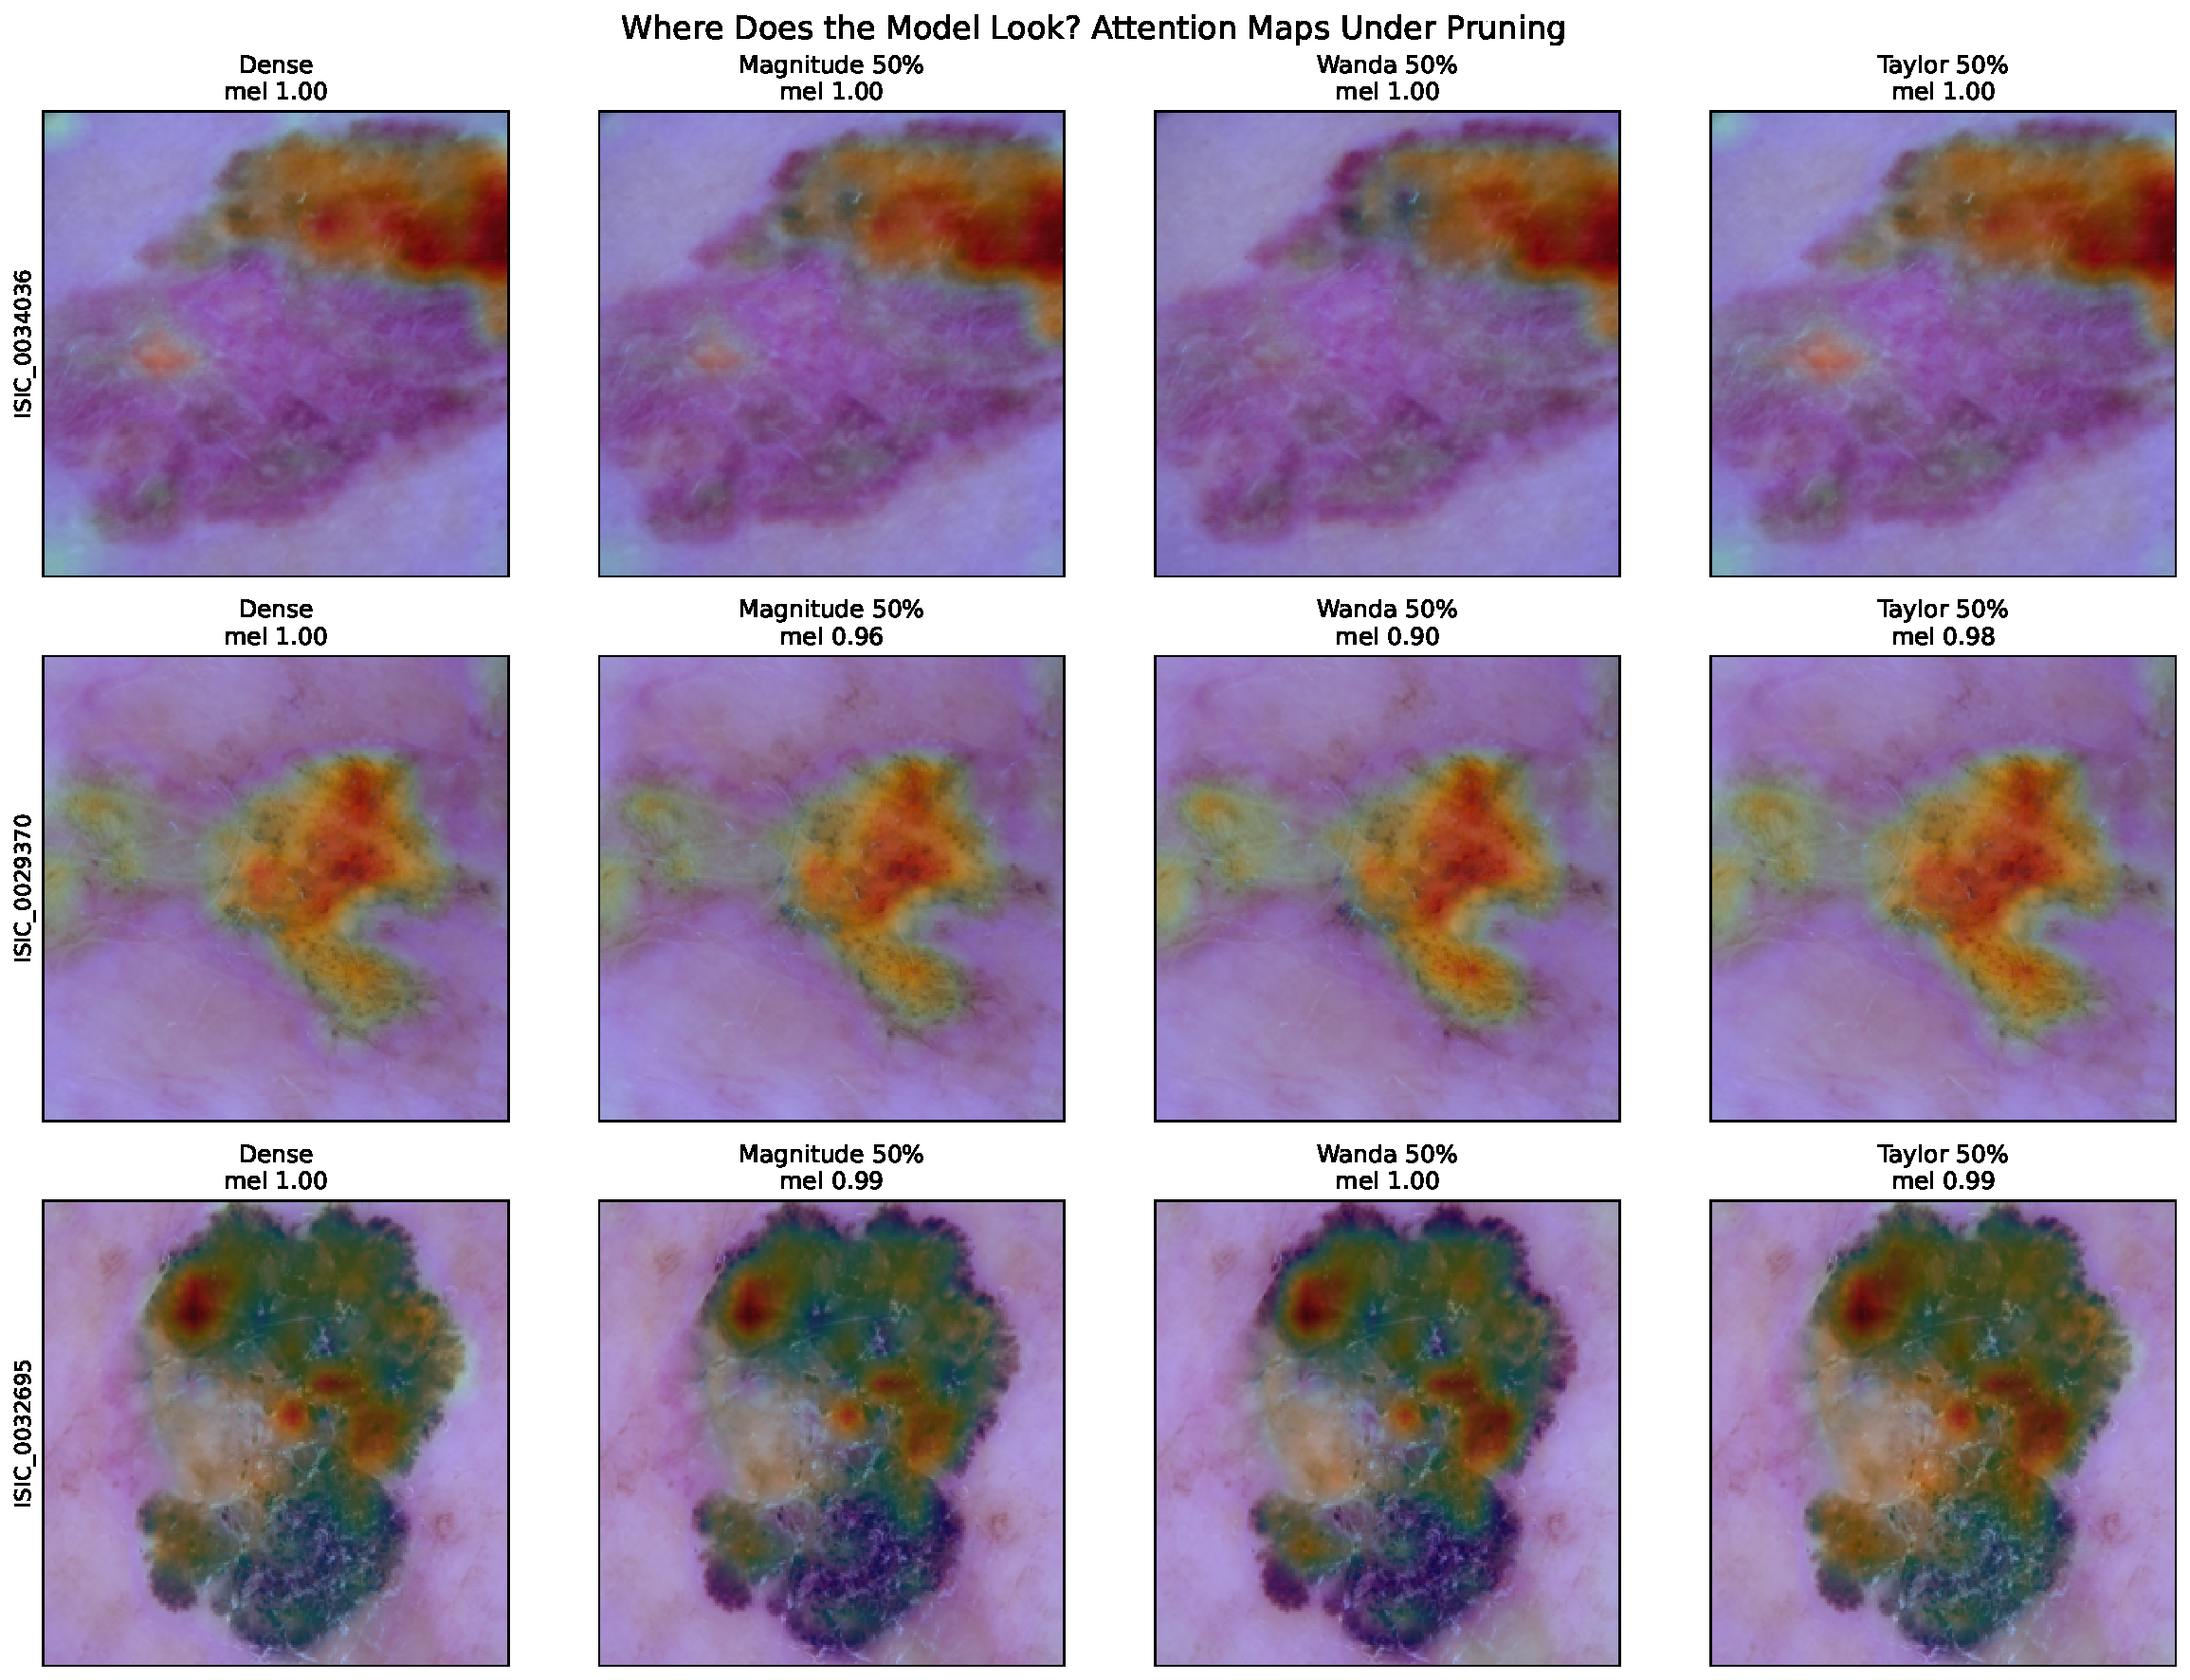
\includegraphics[width=\textwidth]{../results/figures_local/fig8_attention_maps.pdf}
\caption{Attention rollout visualizations for Dense, Magnitude 50\%, Wanda 50\%, and Taylor 50\%. The qualitative pattern is consistent with Table~\ref{tab:attention}: Wanda does not lose lesion localization. Its problem is the downstream classifier behavior, not the ability to attend to the lesion region.}
\label{fig:attention_maps}
\end{figure*}

This matters because it changes what a biomedical team should try to fix. If a compressed model fails because attention maps miss the lesion, then the intervention is architectural or optimization-based. If the model still attends to the lesion but collapses at the classifier head, then the fix is calibration-aware retraining or a different pruning criterion. Our results point to the latter.

\subsection{Sparsity placement and external baselines}
The local exploratory figures and the aggregated non-uniform table tell the same story: where a model is pruned can matter more than the exact score used to rank weights. Sensitivity-guided non-uniform allocation can rescue Wanda, but not every policy helps. In particular, the best Wanda rescue is not the default binned policy alone; the more aggressive binned\_k5 setting reaches balanced accuracy of $0.857$ and melanoma sensitivity of $0.741$, while the learnable policy reaches $0.871$ balanced accuracy but with a higher \DCR{}. The continuous-temperature policies are less stable and should not be the first choice if the goal is a safe clinical default.

\begin{figure}[t]
\centering
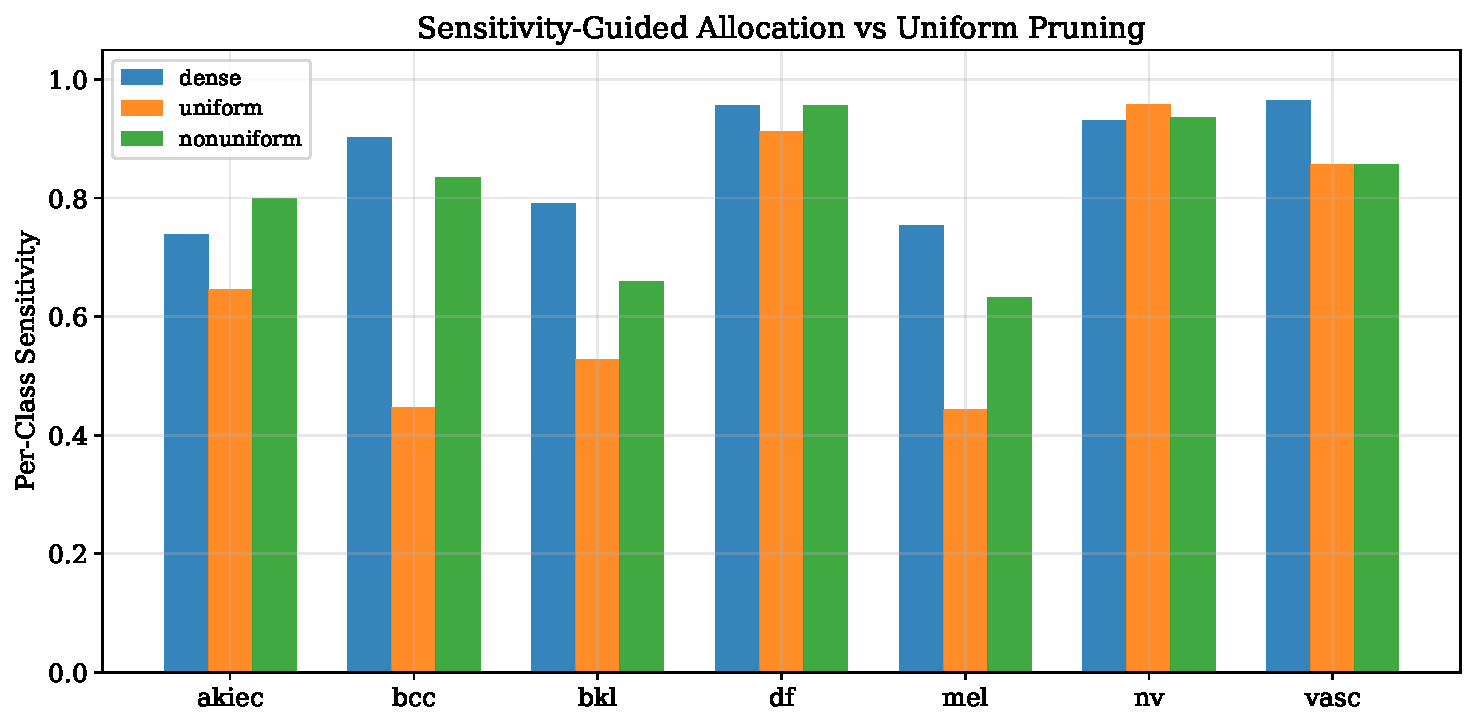
\includegraphics[width=\linewidth]{../results/figures_local/fig4_nonuniform_vs_uniform.pdf}
\caption{Sensitivity-guided non-uniform pruning from the exploratory run. The rescue is obvious for Wanda: redistributing sparsity by layer sensitivity restores a large fraction of the lost class recall. The same idea does not help magnitude nearly as much, which suggests the scoring rule and the sparsity allocation rule should be evaluated together.}
\label{fig:nonuniform}
\end{figure}

External baselines reinforce the main ordering. Paxton-style skewness pruning and X-Pruner are both useful references, but they do not overturn the core finding that Taylor is the best sparse default and that magnitude is not the safest choice for biomedical deployment. X-Pruner is the strongest external 50\% baseline on DeiT-Small if one only looks at balanced accuracy, but Taylor still gives the better melanoma-sensitivity/calibration blend. SparseGPT-pseudo is the clearest poor fit for this medical task. We summarize the detailed non-uniform and baseline results in the appendix because they are valuable implementation guidance but not the main claim of the paper.

\subsection{Quantization, distillation, and the deployment story}
The deployment message is straightforward: start with INT8 quantization, then decide whether sparsity is necessary. Quantization changes the size of the model without changing the structure of the learned function, so it is the least risky compression stage. By contrast, pruning changes which learned connections survive, so the choice of pruning criterion matters.

Knowledge distillation is not a substitute for sparse robustness. In the auxiliary experiments, distillation improved the dense student in some runs, but the pruned distilled student was not reliably better than the directly fine-tuned one. That is the important lesson for biomedical deployment: a better dense baseline does not automatically produce a better compressed model.

Under the conservative clinical thresholds in the log companion files, every evaluated pipeline remains \texttt{academic\_only}. That is not a failure of the paper; it is the honest biomedical reading. The current experiments are strong enough to rank compression choices, but not strong enough to claim unsupervised clinical readiness. On the same host, dense DeiT-Tiny runs at 11.61 ms on CPU and 2.57 ms on MPS, while dense DeiT-Small in the quantization run measures 20.3 ms mean latency and 22.0 ms at p95. Those numbers are the right scale for an edge deployment discussion: they show that the host is fast enough for interactive use, but they do not change the ranking that makes INT8 the safest first size reduction.

\begin{table*}[t]
\centering
\small
\caption{Selected deployment summary from the multi-seed personal quantization run. Quantization preserves the dense behavior closely, but the pruning criterion still determines the downstream clinical tradeoff. Size is reported because it is the primary deployment win; latency is backend-dependent and therefore discussed separately in the appendix.}
\label{tab:quant}
\resizebox{\textwidth}{!}{%
\begin{tabular}{lccccc}
\toprule
Configuration & Bal.\ Acc. & Mel.\ Sens. & Mel.\ AUROC & ECE & Size (MB) \\
\midrule
Dense                & $0.849 \pm 0.069$ & $0.864 \pm 0.077$ & $0.947 \pm 0.026$ & $0.038 \pm 0.015$ & $84.7$ \\
Quantized only       & $0.867 \pm 0.072$ & $0.890 \pm 0.077$ & $0.956 \pm 0.024$ & $0.031 \pm 0.017$ & $22.5$ \\
Magnitude 50\%       & $0.775 \pm 0.060$ & $0.585 \pm 0.057$ & $0.877 \pm 0.024$ & $0.038 \pm 0.006$ & $43.2$ \\
Magnitude 50\% + INT8 & $0.770 \pm 0.061$ & $0.611 \pm 0.073$ & $0.874 \pm 0.024$ & $0.038 \pm 0.008$ & $22.5$ \\
Wanda 50\%           & $0.602 \pm 0.011$ & $0.566 \pm 0.018$ & $0.845 \pm 0.013$ & $0.095 \pm 0.007$ & $43.2$ \\
Wanda 50\% + INT8    & $0.599 \pm 0.012$ & $0.555 \pm 0.023$ & $0.841 \pm 0.012$ & $0.090 \pm 0.007$ & $22.5$ \\
\bottomrule
\end{tabular}}
\end{table*}

Table~\ref{tab:quant} is the practical deployment answer for teams that need a smaller model quickly. INT8 gives the big size win. Taylor remains the better sparse choice. Wanda can be made acceptable only when recall is the overriding goal and calibration is re-checked afterwards.

\section{Discussion and Practical Guidance}
The main lesson is that biomedical compression should be judged by clinical behavior, not by aggregate accuracy alone. Three practical implications follow.

\begin{itemize}[leftmargin=*,itemsep=2pt,topsep=2pt]
  \item \textbf{Use lesion-grouped splits.} Image-level splitting is too optimistic for dermoscopy because the same lesion can appear multiple times.
  \item \textbf{Report the full safety tuple.} Balanced accuracy, melanoma AUROC, ECE, and \DCR{} should be interpreted together. Sensitivity alone is not enough.
  \item \textbf{Start with INT8, then choose sparsity.} Quantization is the lowest-risk compression stage. If sparsity is required, Taylor is the safest default in this study.
  \item \textbf{Treat Wanda non-uniformly.} Wanda can be rescued by non-uniform sparsity, but that makes it a recall-first option, not a universal improvement.
  \item \textbf{Do not assume distillation fixes pruning.} A stronger dense student is not automatically a more pruning-robust student.
  \item \textbf{Validate on the target device.} Latency, calibration, and operating points should be measured on the actual deployment runtime, not assumed from parameter count.
  \item \textbf{Treat the current pipelines as research-only.} Under the conservative clinical thresholds used here, every evaluated configuration remains \texttt{academic\_only}; that is the right interpretation for this study.
\end{itemize}

From a biomedical integration standpoint, the recommendation is conservative but usable: if you can afford only one compression step, use INT8. If you need sparsity, use Taylor and validate the operating point that matters clinically. If you are tempted to use activation-aware Wanda because it looks recall-friendly, check calibration and false positives before you ship.

\section{Limitations}
\begin{itemize}[leftmargin=*,itemsep=2pt,topsep=2pt]
  \item The core claim is established on one dataset and one modality. HAM10000 is a strong case study, not a universal law.
  \item Some auxiliary experiments are exploratory follow-ups from the local run. They are useful for implementation guidance, but they are not the basis of the main pruning claim.
  \item The recovery and calibration follow-ups are informative but not decisive. They show how little the ranking changes under these extra knobs, which is itself a useful deployment lesson.
  \item The paper does not make a second-cohort generalization claim. That would need a separate study.
\end{itemize}

\section{Conclusion}
Compression in biomedical vision is not only a size problem. It is a safety problem. On HAM10000, the failure mode depends on how the model is compressed: magnitude pruning is the least safe baseline, Wanda can look good on sensitivity while degrading calibration and discrimination, and Taylor is the strongest sparse default in the present study. INT8 quantization is the safest first compression stage, and the auxiliary experiments show that recovery, distillation, and calibration size tweaks do not overturn the basic ranking.

The practical result is a deployment recipe, not a new algorithm: use lesion-grouped splits, report clinical metrics together, start with INT8, and use Taylor when you need sparsity. That is a more useful answer for biomedical integration than novelty alone.

\appendix
\section{Layer-Wise Mechanism and Negative Results}
The per-layer analysis in Figure~\ref{fig:perlayer} is useful because it points to the layers that matter most for diagnostic behavior. The local exploratory run shows that the MLP blocks are the most damage-sensitive components, while patch embedding is comparatively stable. This matches the intuition that the model's class-conditional behavior lives in the middle and late transformer blocks rather than in the very first projection.

We also checked an activation-outlier hypothesis: the idea that Wanda's behavior could be explained by a simple relationship between heavy-tailed activation statistics and the damage induced by pruning. The project summary reports that those correlations are near zero. That is a negative result, but it is valuable because it rules out the most obvious story and prevents us from overfitting a false mechanism.

\section{Non-Uniform Allocation and External Baselines}
Table~\ref{tab:nonuniform} shows the non-uniform allocation results from the multi-seed personal aggregate. The core pattern is simple: binned non-uniform sparsity can rescue Wanda, while a continuous-temperature rule is much less stable. The point is not that a cleverer allocation policy always wins. The point is that sparsity placement interacts with the pruning criterion.

\begin{table*}[t]
\centering
\small
\caption{Non-uniform allocation on DeiT-Small at 50\% average sparsity. The binned policy is the one that most clearly rescues Wanda; the continuous policy is less stable.}
\label{tab:nonuniform}
\resizebox{\textwidth}{!}{%
\begin{tabular}{lllccc}
\toprule
Criterion & Policy & Bal.\ Acc. & Mel.\ Sens. & Mel.\ AUROC & \DCR \\
\midrule
Magnitude & uniform         & $0.787 \pm 0.025$ & $0.569 \pm 0.053$ & $0.881 \pm 0.019$ & $1.87 \pm 0.42$ \\
Magnitude & binned\_default & $0.758 \pm 0.047$ & $0.452 \pm 0.064$ & $0.858 \pm 0.034$ & $2.50 \pm 0.87$ \\
Magnitude & continuous\_t1  & $0.652 \pm 0.120$ & $0.240 \pm 0.119$ & $0.793 \pm 0.047$ & $2.14 \pm 1.35$ \\
Wanda     & uniform         & $0.612 \pm 0.018$ & $0.539 \pm 0.041$ & $0.837 \pm 0.019$ & $0.77 \pm 0.09$ \\
Wanda     & binned\_default & $0.841 \pm 0.036$ & $0.727 \pm 0.068$ & $0.918 \pm 0.012$ & $2.62 \pm 0.61$ \\
Wanda     & continuous\_t1  & $0.755 \pm 0.075$ & $0.579 \pm 0.110$ & $0.891 \pm 0.045$ & $2.58 \pm 3.26$ \\
\bottomrule
\end{tabular}}
\end{table*}

The external baseline zoo is useful mostly because it anchors the main ranking. Paxton-style skewness pruning and X-Pruner are both reasonable comparators, but neither overturns the main result that Taylor is the strongest sparse default in this study.

\begin{table}[t]
\centering
\small
\caption{External pruning baselines on the multi-seed aggregate. The values are useful as anchors, but they do not change the main ranking.}
\label{tab:baselines}
\begin{tabular}{llccc}
\toprule
Model & Method & Bal.\ Acc. & Mel.\ Sens. & \DCR \\
\midrule
\multirow{3}{*}{DeiT-Small}
 & Paxton (50\%)  & 0.631 & 0.388 & 1.46 \\
 & X-Pruner (50\%) & 0.747 & 0.746 & 1.58 \\
 & SparseGPT (50\%) & 0.208 & 0.000 & 1.14 \\
\midrule
\multirow{3}{*}{DeiT-Tiny}
 & Paxton (50\%)  & 0.616 & 0.529 & 1.23 \\
 & X-Pruner (50\%) & 0.644 & 0.750 & 0.34 \\
 & SparseGPT (50\%) & 0.227 & 0.067 & 0.85 \\
\bottomrule
\end{tabular}
\end{table}

\section{Quantization, Distillation, and Edge Deployment}
The quantization story is simple: INT8 preserves the dense model's clinical behavior closely while cutting size by roughly 3.8$\times$. The stack results show that pruning, not quantization, is the dominant source of degradation. That makes quantization the safest first compression stage.

\begin{table*}[t]
\centering
\small
\caption{Selected quantization-stacking results from the personal multi-seed runs. Quantization is the safest size reduction, but pruning still controls the clinical tradeoff. Latency is backend-dependent and therefore not the main recommendation signal.}
\label{tab:stacking}
\resizebox{\textwidth}{!}{%
\begin{tabular}{lcccccc}
\toprule
Configuration & Bal.\ Acc. & Mel.\ Sens. & Mel.\ AUROC & Macro AUROC & ECE & Size (MB) \\
\midrule
Dense                & $0.849 \pm 0.069$ & $0.864 \pm 0.077$ & $0.947 \pm 0.026$ & $0.971 \pm 0.018$ & $0.038 \pm 0.015$ & $84.7$ \\
Quantized only       & $0.867 \pm 0.072$ & $0.890 \pm 0.077$ & $0.956 \pm 0.024$ & $0.977 \pm 0.016$ & $0.031 \pm 0.017$ & $22.5$ \\
Magnitude 50\%       & $0.775 \pm 0.060$ & $0.585 \pm 0.057$ & $0.877 \pm 0.024$ & $0.954 \pm 0.015$ & $0.038 \pm 0.006$ & $43.2$ \\
Magnitude 50\% + INT8 & $0.770 \pm 0.061$ & $0.611 \pm 0.073$ & $0.874 \pm 0.024$ & $0.953 \pm 0.016$ & $0.038 \pm 0.008$ & $22.5$ \\
Wanda 50\%           & $0.602 \pm 0.011$ & $0.566 \pm 0.018$ & $0.845 \pm 0.013$ & $0.918 \pm 0.009$ & $0.095 \pm 0.007$ & $43.2$ \\
Wanda 50\% + INT8    & $0.599 \pm 0.012$ & $0.555 \pm 0.023$ & $0.841 \pm 0.012$ & $0.917 \pm 0.009$ & $0.090 \pm 0.007$ & $22.5$ \\
\bottomrule
\end{tabular}}
\end{table*}

Figure~\ref{fig:stacking_perclass} makes the point at the per-class level: the ``pruned only'' and ``pruned plus quantized'' bars are nearly identical for every class, while both differ substantially from the dense reference. INT8 does not perturb the per-class sensitivity profile that pruning has already set.

\begin{figure}[t]
\centering
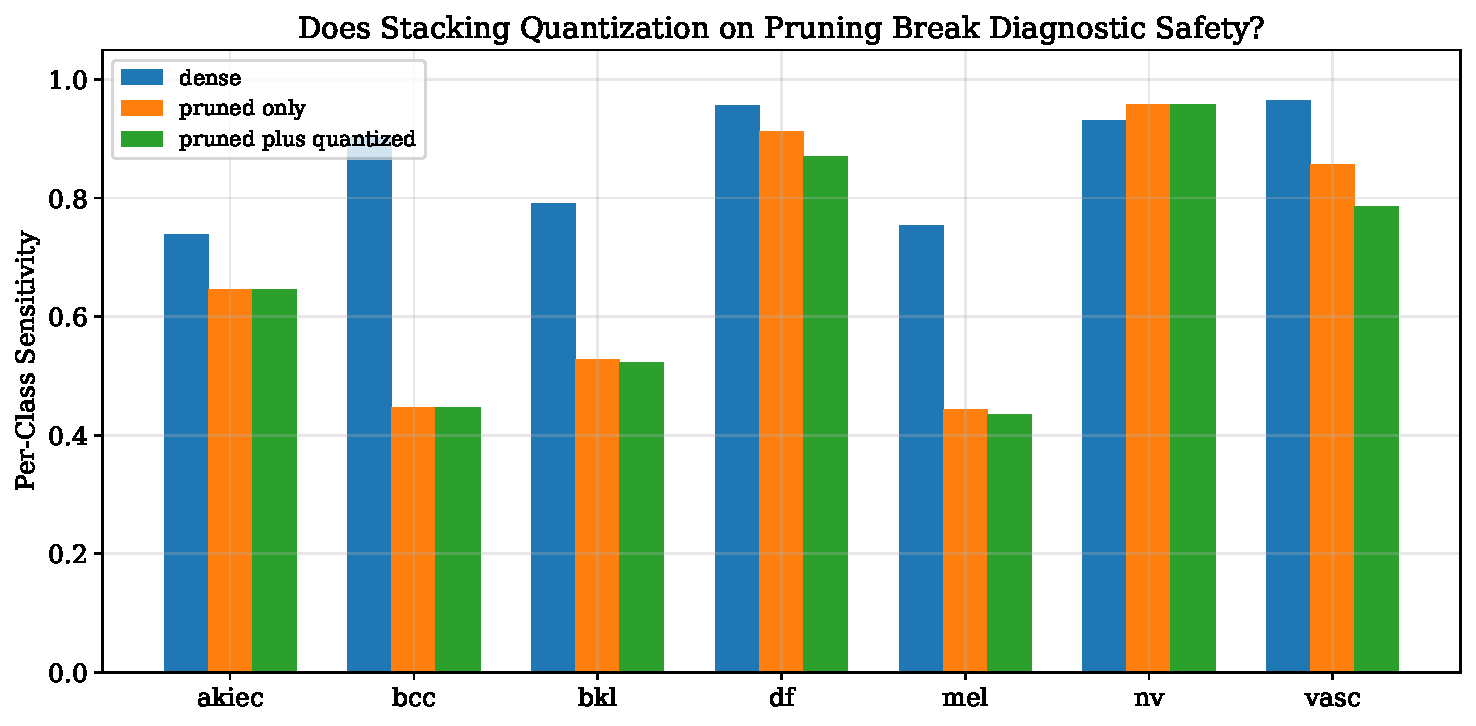
\includegraphics[width=\linewidth]{../results/figures_local/fig5_stacking.pdf}
\caption{Per-class sensitivity for dense, pruned, and pruned plus INT8 quantized DeiT-Small at 50\% magnitude sparsity. The pruned and pruned-plus-quantized bars track each other class by class, including on dangerous classes (\akiec, \bcc, \mel). This is the visual version of the claim that pruning, not quantization, drives the clinical degradation.}
\label{fig:stacking_perclass}
\end{figure}

Distillation is a good reminder that a strong dense model is not automatically a strong compressed model. In the multi-seed personal runs, the distilled dense student did not consistently beat the directly fine-tuned dense model, and the distilled pruned student was clearly not pruning-robust. That makes distillation useful as a dense-student regularizer, but not as a universal pre-treatment for sparsity.

\begin{table}[t]
\centering
\small
\caption{Knowledge distillation pre-treatment on DeiT-Tiny. Distillation is not a free robustness boost; pruned distilled models remain fragile.}
\label{tab:kd}
\begin{tabular}{llccc}
\toprule
Variant & Pruned? & Bal.\ Acc. & Mel.\ AUROC & ECE \\
\midrule
Direct    & No  & $0.865 \pm 0.075$ & $0.947 \pm 0.027$ & $0.035 \pm 0.018$ \\
Distilled & No  & $0.795 \pm 0.023$ & $0.928 \pm 0.008$ & $0.033 \pm 0.009$ \\
Direct    & Yes & $0.353 \pm 0.019$ & $0.795 \pm 0.019$ & $0.120 \pm 0.014$ \\
Distilled & Yes & $0.215 \pm 0.029$ & $0.648 \pm 0.059$ & $0.161 \pm 0.032$ \\
Imagenet  & No  & $0.153 \pm 0.014$ & $0.524 \pm 0.072$ & $0.237 \pm 0.060$ \\
Imagenet  & Yes & $0.149 \pm 0.014$ & $0.577 \pm 0.107$ & $0.286 \pm 0.084$ \\
\bottomrule
\end{tabular}
\end{table}

On the deployment side, the only latency numbers that should be treated as stable are the ones measured on the actual target runtime. In the project logs, dense DeiT-Tiny ran at 11.61 ms on CPU and 2.57 ms on MPS on the same host. That is the right kind of evidence for a biomedical deployment argument: honest, device-specific, and directly relevant to the target environment.

\section{Recovery, Calibration, and the CNN Baseline}
Recovery fine-tuning is useful mainly as a ``what does not rescue the model'' check. In the current multi-seed aggregate, the ranking remains largely unchanged across the sweep. Calibration-size ablation is similar: it moves Wanda a little, but it does not change the overall recommendation.

\begin{table*}[t]
\centering
\small
\caption{Recovery sweep on the multi-seed aggregate. The sweep changes the numbers slightly but does not change the ordering.}
\label{tab:recovery}
\begin{tabular}{llcccc}
\toprule
Model & Criterion & Sparsity & Recovery epochs & Bal.\ Acc. & Mel.\ Sens. \\
\midrule
DeiT-Small & Magnitude & 50\% & 5/10/20 & $0.775 \pm 0.074$ & $0.585 \pm 0.070$ \\
DeiT-Small & Taylor    & 50\% & 5/10/20 & $0.746 \pm 0.060$ & $0.874 \pm 0.086$ \\
DeiT-Small & Wanda     & 50\% & 5/10/20 & $0.598 \pm 0.007$ & $0.533 \pm 0.019$ \\
DeiT-Tiny   & Magnitude & 50\% & 5/10/20 & $0.845 \pm 0.084$ & $0.789 \pm 0.059$ \\
DeiT-Tiny   & Taylor    & 50\% & 5/10/20 & $0.836 \pm 0.004$ & $0.700 \pm 0.035$ \\
DeiT-Tiny   & Wanda     & 50\% & 5/10/20 & $0.794 \pm 0.023$ & $0.717 \pm 0.020$ \\
\bottomrule
\end{tabular}
\end{table*}

\begin{figure}[t]
\centering

\includegraphics[width=\linewidth]{../results/figures_personal/fig7_recovery_balacc.pdf}

\includegraphics[width=\linewidth]{../results/figures_personal/fig7_recovery_mel.pdf}
\caption{Recovery fine-tuning on balanced accuracy and melanoma sensitivity. The main lesson is that recovery does not change the criterion ranking enough to alter the biomedical recommendation.}
\label{fig:recovery}
\end{figure}

\begin{table}[t]
\centering
\small
\caption{Calibration-size ablation for Wanda on the multi-seed aggregate. Larger calibration sets help only modestly; they do not turn Wanda into a better sparse default than Taylor.}
\label{tab:calibration}
\begin{tabular}{ccc}
\toprule
Calibration size & Bal.\ Acc. & Mel.\ Sens. \\
\midrule
16  & 0.610 & 0.455 \\
32  & 0.611 & 0.375 \\
64  & 0.612 & 0.410 \\
128 & 0.619 & 0.407 \\
256 & 0.618 & 0.436 \\
512 & 0.611 & 0.408 \\
\bottomrule
\end{tabular}
\end{table}

The MobileNetV2 baseline is an important sanity check because it shows that fragility under unstructured pruning is not unique to transformers. In this project, the CNN baseline collapses more quickly than the ViTs under the same pruning settings. That makes the main recommendation more, not less, relevant: the problem is the compression criterion and the deployment objective, not the architecture label.

\begin{table}[t]
\centering
\small
\caption{MobileNetV2 baseline. This is an exploratory architecture check rather than a generalization claim.}
\label{tab:mobilenet}
\begin{tabular}{lccc}
\toprule
Setup & Bal.\ Acc. & Mel.\ Sens. & Macro AUROC \\
\midrule
Dense      & 0.766 & 0.633 & 0.953 \\
Magnitude 30\% & 0.722 & 0.604 & 0.950 \\
Magnitude 50\% & 0.251 & 0.071 & 0.872 \\
Magnitude 70\% & 0.143 & 0.000 & 0.573 \\
Wanda 30\%     & 0.166 & 0.004 & 0.835 \\
Wanda 50\%     & 0.143 & 0.000 & 0.532 \\
Wanda 70\%     & 0.143 & 1.000 & 0.573 \\
\bottomrule
\end{tabular}
\end{table}

\section{Conclusion}
Compression in biomedical vision should be judged by clinical behavior, not by aggregate accuracy alone. On HAM10000, the dangerous failure mode is not simply that performance drops, but that compression can drop recall on rare harmful classes disproportionately, or can raise melanoma sensitivity while destroying calibration. Our results show that magnitude pruning is the least safe baseline, Taylor is the best sparse default, INT8 quantization is the safest first compression step, and distillation is useful primarily for dense students. The gradient-coupling probe explains why magnitude fails, and the conservative clinical tags keep us from overclaiming deployment readiness: the evaluated pipelines remain research-only. The principal contribution is a deployment-oriented evaluation protocol that biomedical teams can reuse when deciding how, and whether, to compress a model.

\clearpage
\bibliographystyle{plainnat}
\bibliography{references}

\end{document}
